\section{Ellipsoids}

\textbf{(a)}
For a \(2\times 2\) symmetric positive definite matrix \(A\), use the eigendecomposition
\[
A=Q\Lambda Q^T,
\qquad
\Lambda=\mathrm{diag}(\lambda_1,\lambda_2),
\qquad
\lambda_i>0
\]
The boundary of the ellipse
\[
E=\{x\in\mathbb{R}^2\mid x^T A x=1\}
\]
can be parametrized by
\[
x(\theta)=Q
\begin{bmatrix}
1/\sqrt{\lambda_1}&0\\
0&1/\sqrt{\lambda_2}
\end{bmatrix}
\begin{bmatrix}
\cos\theta\\
\sin\theta
\end{bmatrix},
\qquad
0\le \theta\le 2\pi
\]
The code at the end.

\textbf{(b)}
For
\[
A=
\begin{bmatrix}
1&0\\
0&2
\end{bmatrix}
\]
the ellipse equation is
\[
x_1^2+2x_2^2=1
\]
so the semiaxis lengths are \(1\) in the \(x_1\) direction and \(1/\sqrt{2}\) in the \(x_2\) direction.

\begin{figure}[H]
    \centering
    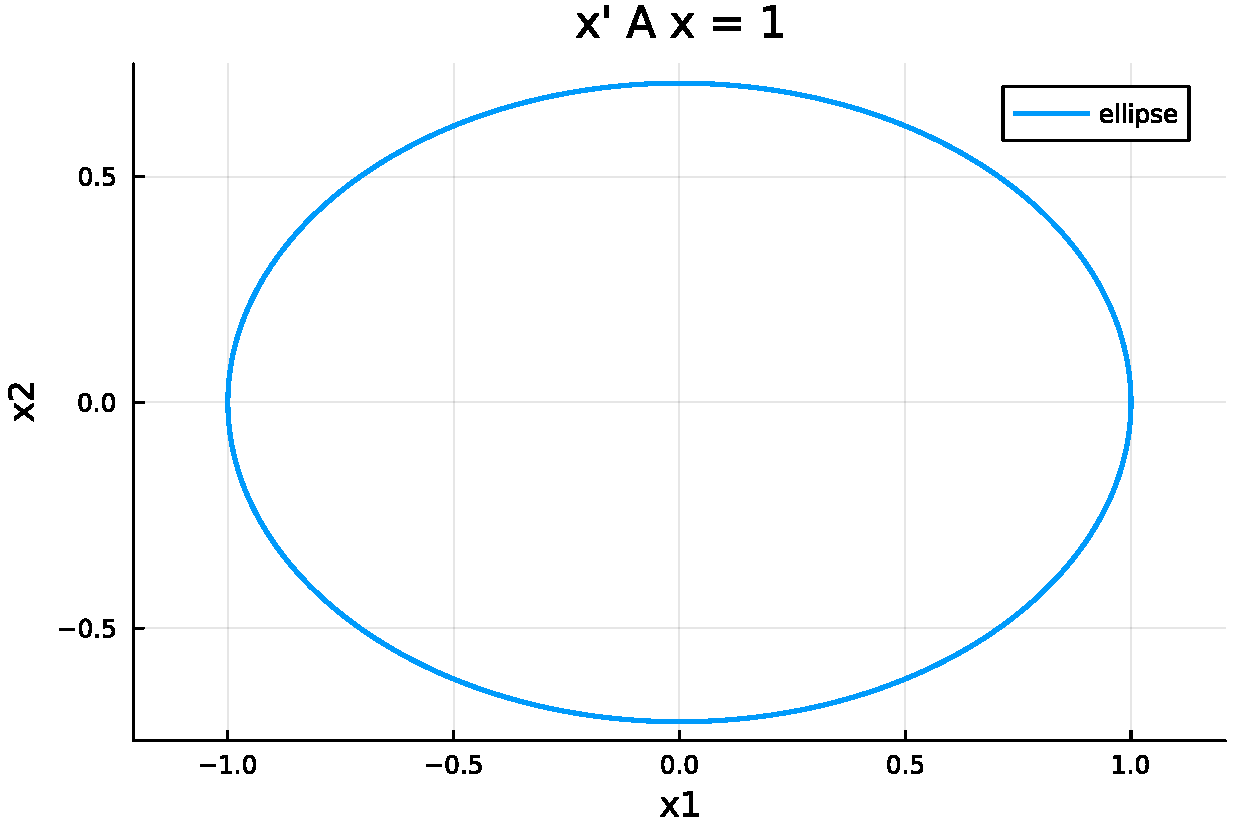
\includegraphics[width=0.72\textwidth]{img/p4b_ellipse.pdf}
    % \caption{Ellipse for \(A=\mathrm{diag}(1,2)\)}
\end{figure}

\textbf{(c)}
For
\[
A=
\begin{bmatrix}
0.2&-0.1\\
-0.1&0.4
\end{bmatrix}
\]
the eigenvalues are
\[
\lambda_1=0.158579,\qquad \lambda_2=0.441421
\]
so the semiaxis lengths are
\[
\frac{1}{\sqrt{\lambda_1}}=2.511179,
\qquad
\frac{1}{\sqrt{\lambda_2}}=1.505128
\]
The corresponding semiaxis directions are approximately
\[
\begin{bmatrix}
-0.923880\\
-0.382683
\end{bmatrix},
\qquad
\begin{bmatrix}
-0.382683\\
0.923880
\end{bmatrix}
\]

\begin{figure}[H]
    \centering
    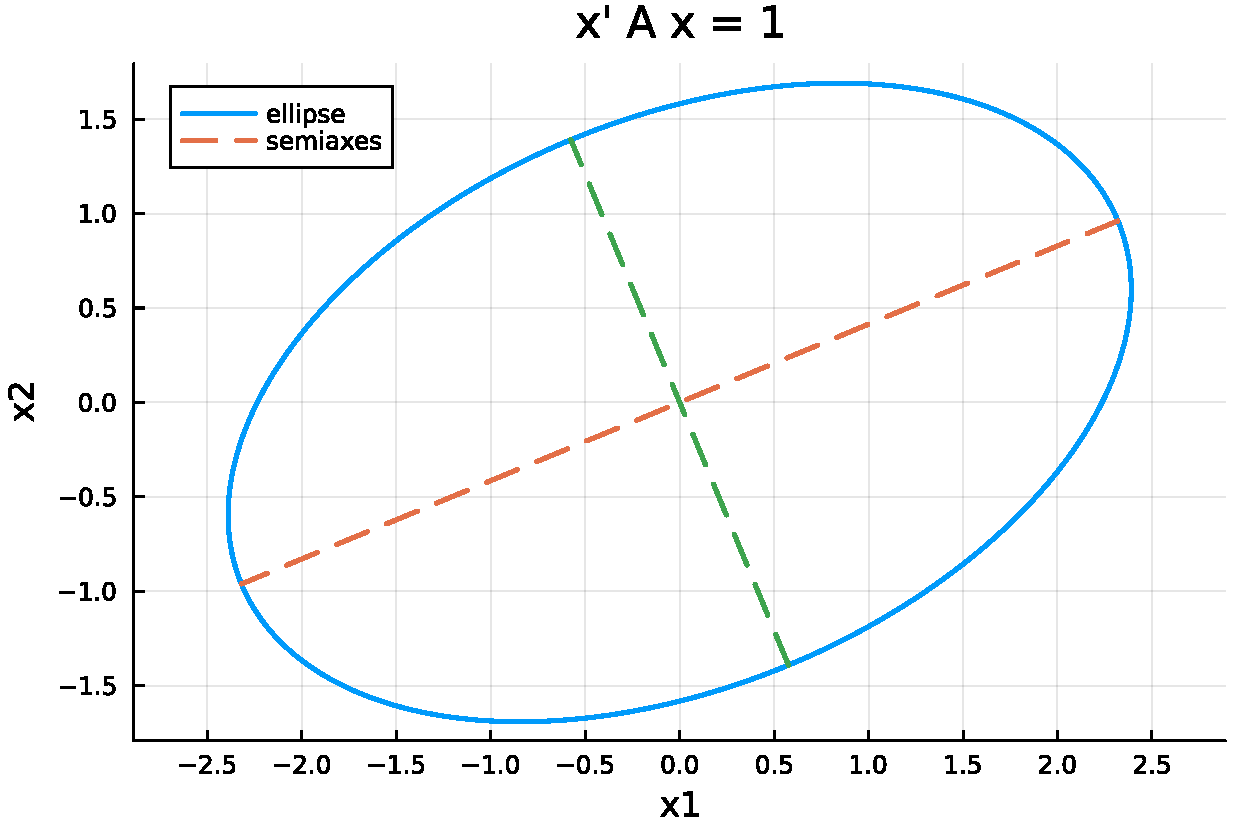
\includegraphics[width=0.72\textwidth]{img/p4c_ellipse.pdf}
    \caption{Ellipse with semiaxes shown}
\end{figure}

\textbf{(d)}
Put the sensor vectors into
\[
B=
\begin{bmatrix}
b_1&b_2&b_3
\end{bmatrix}
\]
Then
\[
y=B^T x
\]
and the set \(\|y\|_2\le 1\) is
\[
\|B^T x\|_2^2\le 1
\]
Equivalently,
\[
x^TBB^T x\le 1
\]
For the given vectors,
\[
BB^T=
\begin{bmatrix}
1.4987&0.2969\\
0.2969&1.4987
\end{bmatrix}
\]
so this set is an ellipse centered at the origin.
The feasible set consists of the interior of the blue ellipse together with its boundary.

\begin{figure}[H]
    \centering
    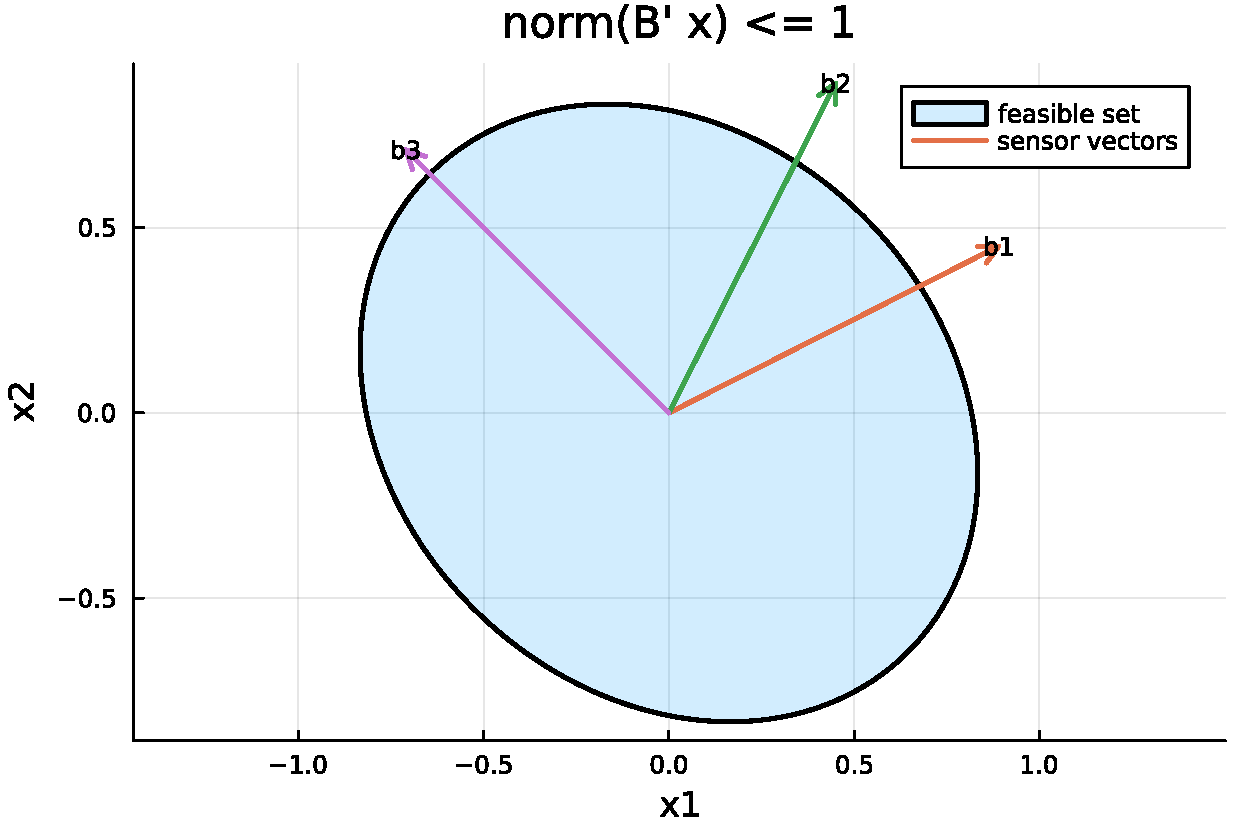
\includegraphics[width=0.72\textwidth]{img/p4d_sensors.pdf}
    % \caption{Set \(\|B^Tx\|_2\le 1\), with sensor vectors shown}
\end{figure}

\subsection{Code}
\begin{lstlisting}[language={}]
using LinearAlgebra
using Plots

function ellipse_points(A; npoints=500)
    E = eigen(Symmetric(A))
    theta = range(0, 2pi, length=npoints)
    circle = hcat(cos.(theta), sin.(theta))'
    points = E.vectors * Diagonal(1 ./ sqrt.(E.values)) * circle
    return points[1, :], points[2, :], E.values, E.vectors
end

function tick_locations(values; step=0.5)
    lower = step * floor(minimum(values) / step)
    upper = step * ceil(maximum(values) / step)
    return lower:step:upper
end

function plot_ellipse(A; show_semiaxes=false, vectors=nothing,
                      fill_feasible=false, tick_step=0.5)
    x, y, vals, vecs = ellipse_points(A)
    p = plot(x, y;
             seriestype=fill_feasible ? :shape : :path,
             aspect_ratio=:equal,
             xticks=tick_locations(x; step=tick_step),
             yticks=tick_locations(y; step=tick_step),
             fillalpha=fill_feasible ? 0.18 : 0.0,
             label=fill_feasible ? "feasible set" : "ellipse")

    if show_semiaxes
        for i in 1:2
            axis = vecs[:, i] / sqrt(vals[i])
            plot!(p, [-axis[1], axis[1]], [-axis[2], axis[2]];
                  linestyle=:dash, label=i == 1 ? "semiaxes" : false)
        end
    end

    if vectors !== nothing
        for i in 1:size(vectors, 2)
            b = vectors[:, i]
            plot!(p, [0.0, b[1]], [0.0, b[2]];
                  arrow=true, label=i == 1 ? "sensor vectors" : false)
        end
    end

    return p
end

A_b = [1.0 0.0;
       0.0 2.0]

A_c = [0.2 -0.1;
       -0.1 0.4]

b1 = [0.89, 0.45]
b2 = [0.45, 0.89]
b3 = [-0.71, 0.71]
B = hcat(b1, b2, b3)
A_d = B * B'

plot_ellipse(A_b)
plot_ellipse(A_c; show_semiaxes=true)
plot_ellipse(A_d; vectors=B, fill_feasible=true)
\end{lstlisting}
